%
% File acl2017.tex
%
%% Based on the style files for ACL-2015, with some improvements
%%  taken from the NAACL-2016 style
%% Based on the style files for ACL-2014, which were, in turn,
%% based on ACL-2013, ACL-2012, ACL-2011, ACL-2010, ACL-IJCNLP-2009,
%% EACL-2009, IJCNLP-2008...
%% Based on the style files for EACL 2006 by 
%%e.agirre@ehu.es or Sergi.Balari@uab.es
%% and that of ACL 08 by Joakim Nivre and Noah Smith

\documentclass[11pt,a4paper]{article}
\usepackage[hyperref]{acl2017}
\usepackage{times}
\usepackage{latexsym}
\usepackage{bm}
\usepackage{graphicx}
\usepackage{amsmath}
\DeclareMathOperator*{\argmax}{argmax} % thin space, limits underneath in displays
\usepackage{url}
\usepackage[inline,shortlabels]{enumitem}
\usepackage{caption}% <-- added

\usepackage{tabularx,booktabs}
\newcolumntype{C}{>{\centering\arraybackslash\hsize=.5\hsize}X} % centered version of "X" type
\setlength{\extrarowheight}{1pt}


\usepackage{adjustbox}
\usepackage{float}



\aclfinalcopy % Uncomment this line for the final submission
%\def\aclpaperid{***} %  Enter the acl Paper ID here

%\setlength\titlebox{5cm}
% You can expand the titlebox if you need extra space
% to show all the authors. Please do not make the titlebox
% smaller than 5cm (the original size); we will check this
% in the camera-ready version and ask you to change it back.

\newcommand\BibTeX{B{\sc ib}\TeX}

\title{CS395T: Neural Networks for Sentiment Analysis Project Report}

\author{Zeyuan Hu \\
  Computer Science Department \\
  University of Texas at Austin \\
  Austin, Texas \\
  {\tt iamzeyuanhu@utexas.edu} \\
}

\date{}

\begin{document}
\maketitle

\begin{abstract}
In this project, I implement a Feedforward Neural Network based on
averaged word vectors over the input sentence and a convolutional neural
network (CNN) to perform the sentiment analysis on the sentences from
Rotten Tomatoes introduced by Pang and Lee~\shortcite{Pang:2005}.
\end{abstract}

\section{Collaborators}
Zhan Shi, Danlu Wang

\section{Introduction}

Sentiment analysis is an umbrella term for several closely-related tasks. One of them is to
classifiy the sentences as either negative or positive. Traditionally, Naive Bayes or SVM
bag-of-words models are well-suited for those tasks. However, neural network approaches
including convolutional networks \cite{Kim14f} and feedforward networks \cite{Iyyer2015} 
can substitute those traditional models to achieve similar performance. In this project,
I implement a feedford network and a convolutional neural networks for the sentiment analysis.
In addition, I explore various architectural and parameter options to 
tune the systems to gain good classification performance.

\section{Implementation Details}

\subsection{Feedforward Neural Networks}

The implementation of the feedforword neural network (FFNN) follows closely to
the architecture of the deep averaging network (DAN)
described by Iyyer et al.~\shortcite{Iyyer2015}. In the paper, the authors
break down the architecture into three simple steps: 1. take the average of
word embeddings of words in a given sentence 2. pass the average into a 
FFNN with one or more hidden layers 3. perform classification
on the final output. I follow those three steps closely and my network contains
one hidden layer. Essentially, I calculate $P(\boldsymbol{y}|\boldsymbol{x})$ in the network.
\verb|one_best| contains the classifiction result of the sentences in the computataion graph \verb|graph|.
I implement batching and during each epoch, I shuffle
the training examples at the very beginning. For the optimizer, I experiment with both the Adam
and the stochastic gradient descent (SGD). The parameter tuning and the impact of the optimizer
to the performance will be disccued in details in the experiment section.

\subsection{CNN}

The implementation of CNN follows Zhang and Wallace~\shortcite{Zhang15}'s empiricial study of
one-layer CNN hyperparameter setting on sentence classification. In my implementation, I use
one convolution layer with multiple filter widths and feature maps and then I use 1-max pooling
suggested in the paper. The code structure is divided into five steps: 
\begin {enumerate*}[1) ]
\item construct embedding layer by looking up pre-trained word embeddings,
\item create convolution layer and implement 1-max pooling strategy, 
\item combine all the pooled features,
\item add dropout, and 
\item make final predictions.
\end {enumerate*} 
The rest of work is to focus on the hyperparameter setting, which
includes filter region size(s) (i.e., \verb|filter_sizes|), 
the number of filters to use with each size (i.e., \verb|num_filters|),
the activation function(s) (i.e., \verb|activation_func|), and so on.

\section{Experiments}

The experiment is carried out in a similar way as Zhang and Wallace~\shortcite{Zhang15}'s.
For each exploration task, I report the mean, minimum, and maximum average 
accuracy values observed over three replications. 

\subsection{Feedforward Neural Networks}

For the FFNN, I explore the impact of the architecture and 
the choice of the optimizer to the system performance. Without special note, the experiments
is based on the hyperparameter setting in table 1.

\begin{table}
\captionsetup{size=footnotesize}
\caption{FFNN Configuration} \label{tab:freq}
%\setlength\tabcolsep{0pt} % let LaTeX compute intercolumn whitespace
\footnotesize\centering
%This table provides the frequencies.

\smallskip 
\begin{tabular*}{\columnwidth}{@{\extracolsep{\fill}}cc}
\toprule
  Description  & Values  \\
\midrule
 batch size & 10      \\
 number of hidden layer & 1 \\
 number of hidden units & 150        \\
 number of epochs & 50        \\
 initial learning rate & 0.1        \\
 decay steps & 10 \\
 learning rate decay factor & 0.99 \\
 optimizer & SGD \\
\bottomrule
\end{tabular*}
\end{table}

\textbf{Optimizer:} I compare the performance between Adam and SGD, which is controlled by
the environment variable \verb|OPT| in the code. One surprising finding is that whether 
supplying \verb|global_step| argument inside the function call \verb|apply_gradients| 
can have impact on the performance of the system . I use tensorflow version 1.3.0 and the result
is shown in table 1.

\begin{table}[!htb]
\captionsetup{size=footnotesize}
\caption{Optimizer Performance with ``global\_step"} \label{tab:freq}
\setlength\tabcolsep{0pt} % let LaTeX compute intercolumn whitespace
\footnotesize\centering
%This table provides the frequencies.

\smallskip 
\begin{tabular*}{\columnwidth}{@{\extracolsep{\fill}}rccr}
\toprule
  Optimizer  & Arg & Accuracy (training) & Accuracy (dev) \\
\midrule
 SGD & Yes   & 76.53 (76.44, 76.59)    & 74.83 (74.67, 75.05)      \\
 ADAM & Yes   & 77.58 (76.72, 78.23)    & \textbf{74.98 (74.48, 75.33)}     \\
 SGD & No  & \textbf{81.72 (81.15, 82.70)}     & 74.42 (74.20, 74.77)      \\
 ADAM & No   & 50.06 (50.06, 50.06)     & 49.06 (49.06, 49.06)      \\
\bottomrule
\end{tabular*}
\end{table}

As shown in the table, \verb|global_step| does not have impact for SGD
measured by the accuracy on the dev set. Adam has similar performance
as SGD with \verb|global_step|. However, without \verb|global_step|,
Adam performs poorly and SGD has significant increase in training set
accuracy compared with \verb|global_step| unset case.

\textbf{Architecture:} The architecture of FFNN is determined by the number of 
hidden layers. In this experiment, I explore the FFNN with zero and one
hidden layers. The result is shown in table 3. 

\begin{table}[!htb]
\captionsetup{size=footnotesize}
\caption{FFNN architecture} \label{tab:freq}
\setlength\tabcolsep{0pt} % let LaTeX compute intercolumn whitespace
\footnotesize\centering
%This table provides the frequencies.

\smallskip 
\begin{tabular*}{\columnwidth}{@{\extracolsep{\fill}}rcr}
\toprule
  Hidden layers  &  Accuracy (training) & Accuracy (dev) \\
\midrule
 0   &  71.73 (66.66, 77.40)   &  69.48 (65.76, 73.92)     \\
 1    & \textbf{81.72 (81.15, 82.70)}    & \textbf{74.42 (74.20, 74.77)}     \\
 2   & 51.22 (49.94, 52.05)     & 51.88 (50.38, 53.00)     \\
\bottomrule
\end{tabular*}
\end{table}

As shown in the table, there is a significant performance gain 
when we increase our hidden layer from zero to one. However, with
the given configuration, two layers architecture has notable performance
drop. This suggests that hyperparameter setting and architecture has
to be carefully picked to achieve good performance.

%
%\begin{table*}
%\caption{Impact of the parameters on the UAS score}
%\label{data-table}
%\begin{tabularx}{\textwidth}{@{}l*{8}{C}c@{}}
%\toprule
%Parser    & Optimizer & Learning Rate & Epoches & Sentences     & Batch Size     & UAS    \\    
%\midrule
%Greedy    & SGD        & 0.2              & 10         & 5000          & 1         & 72.27  \\    
%Greedy    & SGD        & 0.2            & 20      & 5000           & 1                & 74.67  \\   
%Greedy    & SGD       & 0.2             & 30        & 5000          & 1               & 75.81  \\   
%Greedy    & SGD       & 0.2              & 40         & 5000         & 1               & 75.74  \\   
%\addlinespace
%Greedy    & SGD       & 0.2              & 30         & 6000          & 1              & 76.35  \\   
%Greedy    & SGD       & 0.2              & 30      & 7000         & 1               & 76.43  \\  
%Greedy    & SGD       & 0.2              & 30      & 39832          & 1                & \textbf{78.60}  \\    
%Global    & Adagrad(0.0001, 5) & 5    & 10      & 39832          & 20               & \textbf{75.67}  \\ 
%\bottomrule
%\end{tabularx}
%\end{table*} 

\subsection{CNN}

For the CNN, I explore the impact of the hyperparameter setting to the system performance. 
Without special note, the experiments is based on the configuration in table 4. Figure 1
shows the performance of the CNN versus the number of epochs.

\begin{figure}[h]
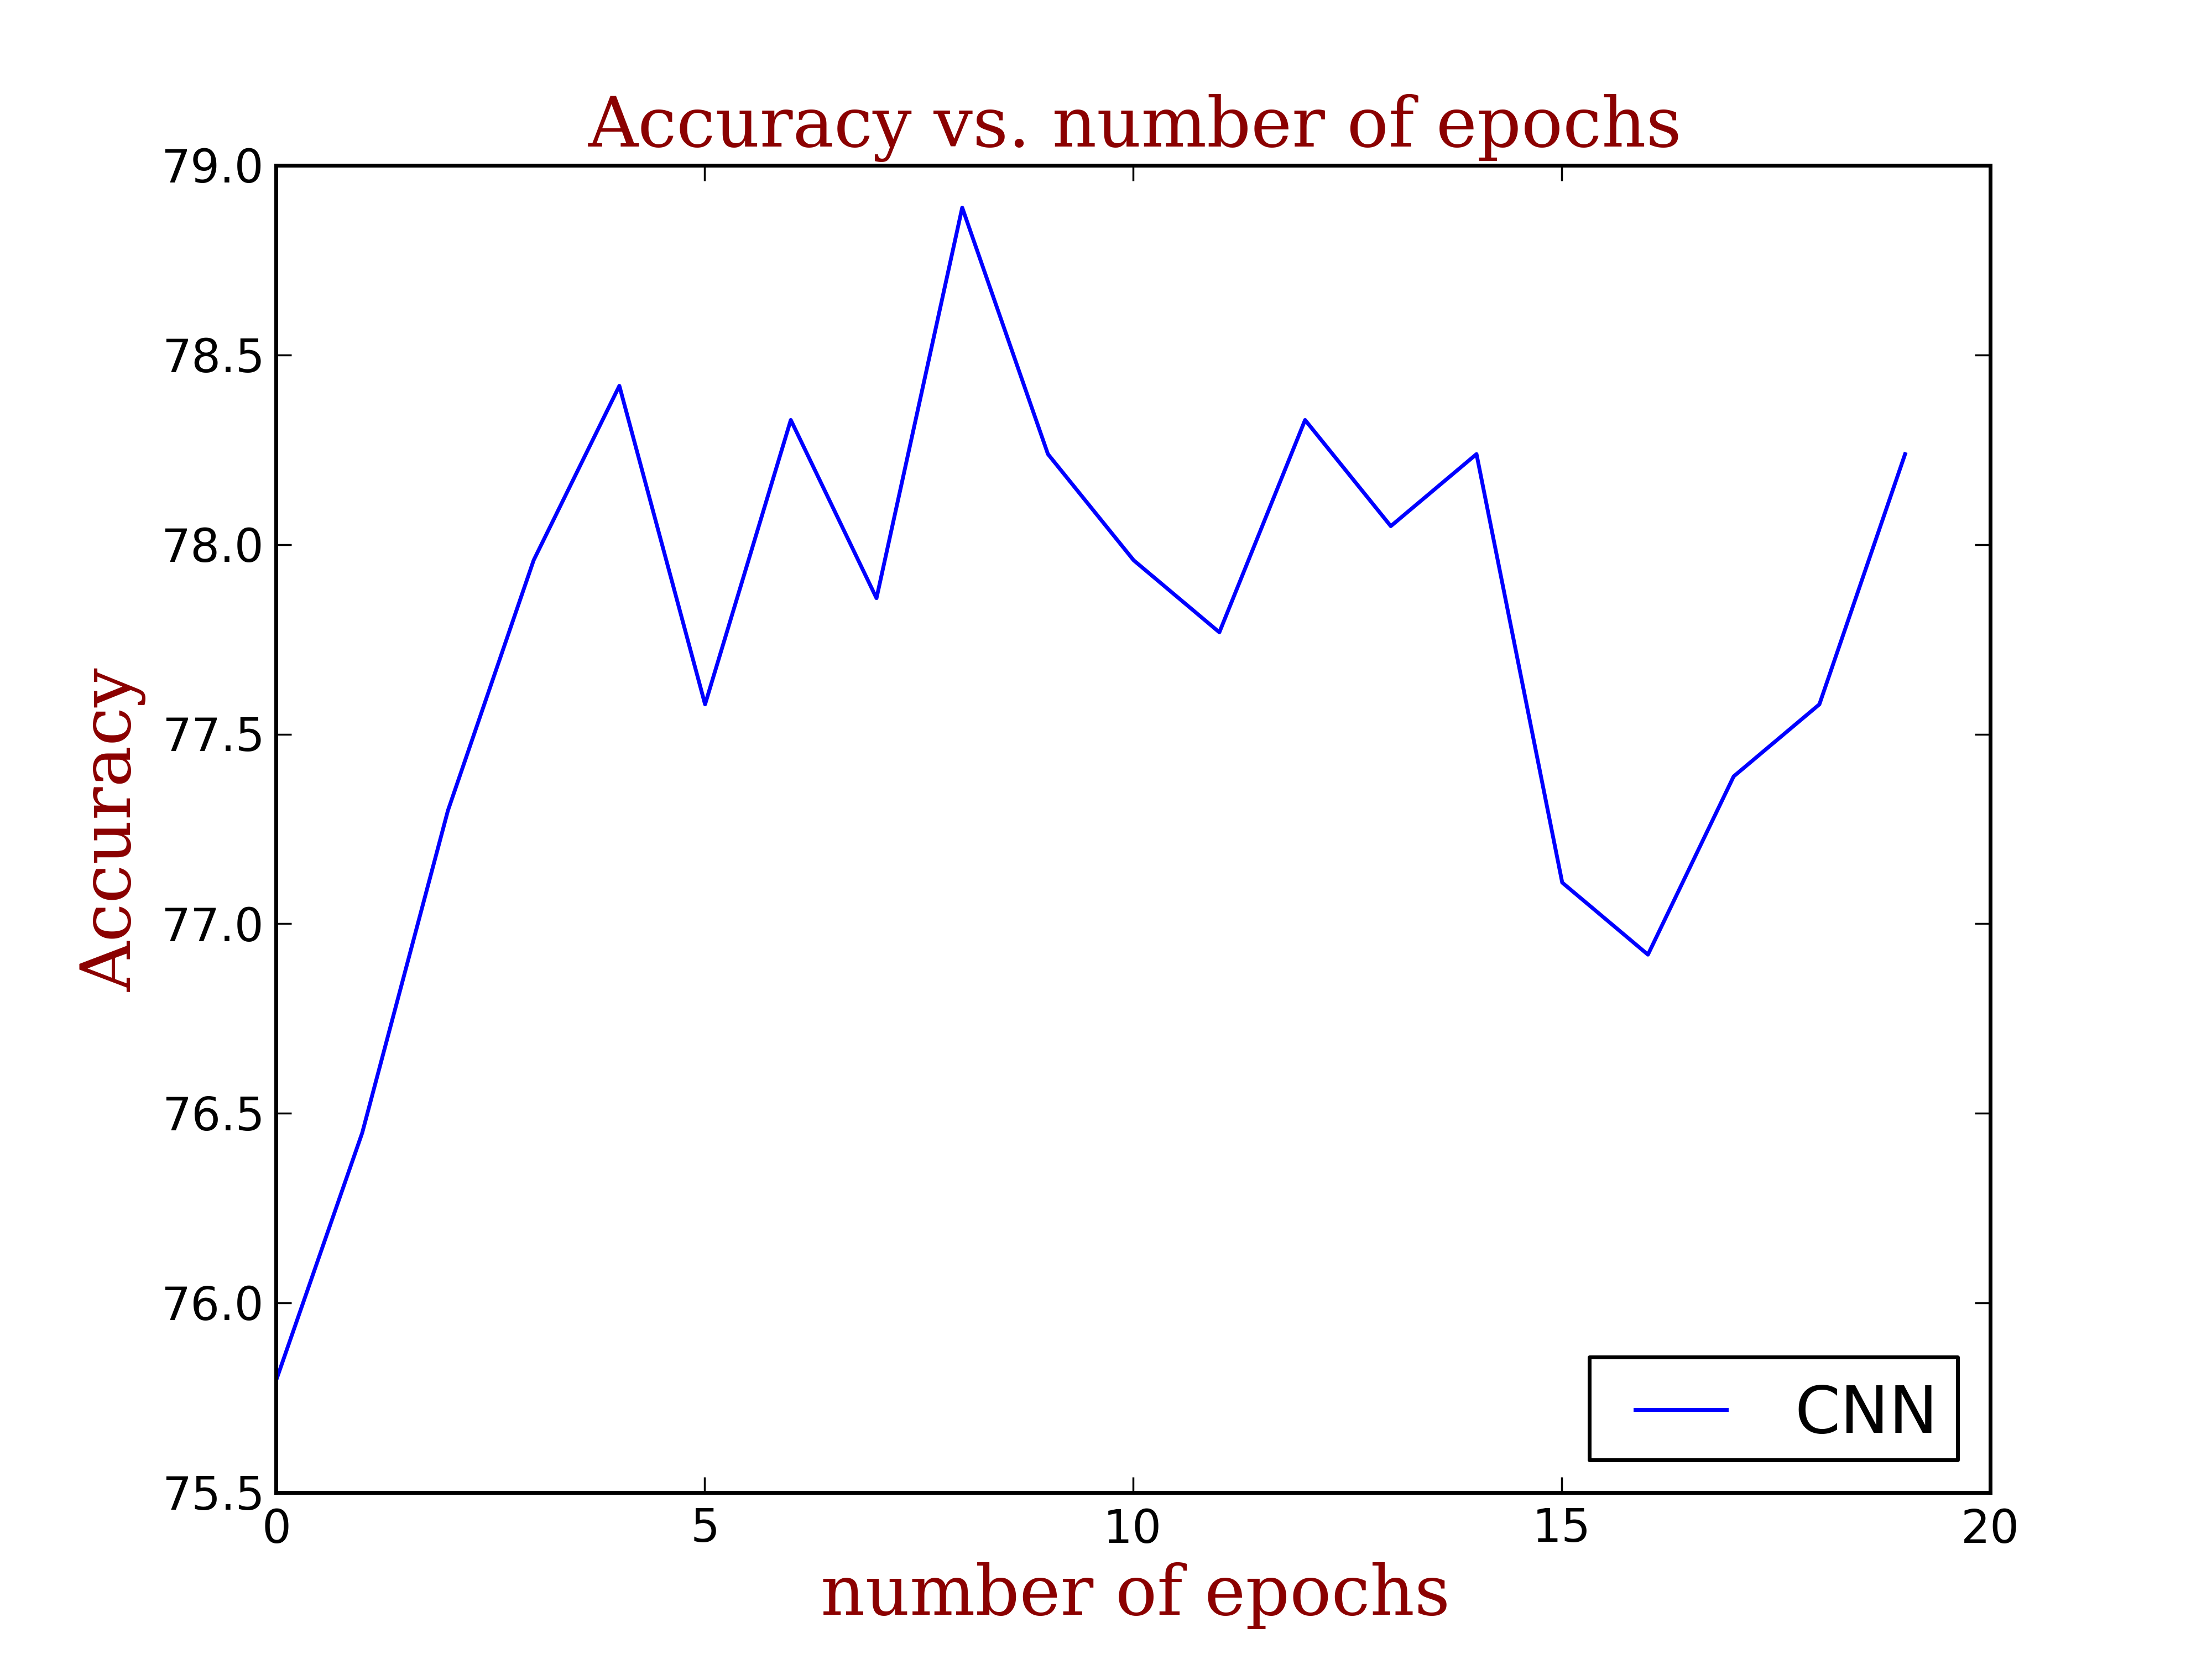
\includegraphics[scale=0.5]{cnn-epoch.png}
\caption{Accuracy vs. number of epochs in dev set}
\end{figure}

\begin{table}
\captionsetup{size=footnotesize}
\caption{CNN Configuration}
%\setlength\tabcolsep{0pt} % let LaTeX compute intercolumn whitespace
\footnotesize\centering
%This table provides the frequencies.

\smallskip 
\begin{tabular*}{\columnwidth}{@{\extracolsep{\fill}}cc}
\toprule
  Description  & Values  \\
\midrule
input word vectors & GloVe-300      \\
filter region size & (3,4,5) \\
feature maps &    128    \\
activation functions & ReLU        \\
pooling & 1-max pooling        \\
dropout rate & 0.5 \\
$l2$ norm constant & 0 \\
optimizer & Adam \\
number of epochs & 20 \\
batch size & 64 \\
\bottomrule
\end{tabular*}
\end{table}

In the following experiments, I train the CNN for $5$ epochs. 
\textbf{Filter region size(s):}
In this experiment, I examine whether the filter region sizes will have
the impact on the CNN performance. The choice of filter region sizes are 
picked based on Zhang and Wallace~\shortcite{Zhang15}'s empirical study. 
The result is shown in table 5. 

\begin{table}[!htb]
\captionsetup{size=footnotesize}
\caption{Filter region sizes and CNN performance} \label{tab:freq}
\setlength\tabcolsep{0pt} % let LaTeX compute intercolumn whitespace
\footnotesize\centering
%This table provides the frequencies.

\smallskip 
\begin{tabular*}{\columnwidth}{@{\extracolsep{\fill}}cc}
\toprule
  Filter region sizes  &   Accuracy (dev) \\
\midrule
(3,4,5)    &  \textbf{77.52 (77.39, 77.77)}     \\
(7,7,7,7)  &  77.20 (76.92, 77.58)     \\
(7)        &  76.92 (76.08, 77.39)     \\
\bottomrule
\end{tabular*}
\end{table}

I try different region sizes and find out that the impact of the region sizes
to the performance is not significant. Even we have one region size $7$, there
is almost no performance drop.

\textbf{Feature maps:}
Zhang and Wallace~\shortcite{Zhang15} suggests that the number of feature maps
for each filter region size is ranged between $100$ and $600$. This is quite large
range. I experiment with three feature maps with one value between $100$ and $200$,
one value between $200$ and $400$, and one value between $400$ and $600$. The result is
shown in table 6.

\begin{table}[!htb]
\captionsetup{size=footnotesize}
\caption{Feature maps and CNN performance} \label{tab:freq}
\setlength\tabcolsep{0pt} % let LaTeX compute intercolumn whitespace
\footnotesize\centering
%This table provides the frequencies.

\smallskip 
\begin{tabular*}{\columnwidth}{@{\extracolsep{\fill}}cc}
\toprule
  Feature maps  &   Accuracy (dev) \\
\midrule
128    &  77.52 (77.39, 77.77)     \\
300  &    \textbf{77.86 (77.67, 78.05)} \\
600    &  77.61 (76.83, 78.52)    \\
\bottomrule
\end{tabular*}
\end{table}

\textbf{Activation functions:}
In this experiment, I experiment with two activation functions: \verb|tanh| and \verb|relu|.
The result is summarized in the table 7.

\begin{table}[!htb]
\captionsetup{size=footnotesize}
\caption{Activation functions and CNN performance} \label{tab:freq}
\setlength\tabcolsep{0pt} % let LaTeX compute intercolumn whitespace
\footnotesize\centering
%This table provides the frequencies.

\smallskip 
\begin{tabular*}{\columnwidth}{@{\extracolsep{\fill}}cc}
\toprule
  Activation function  &   Accuracy (dev) \\
\midrule
 \verb|tanh|   &   77.49 (77.30, 77.77)     \\
 \verb|relu|    &  \textbf{77.52 (77.39, 77.77)}     \\
\bottomrule
\end{tabular*}
\end{table}

As shown in the table 7, the choice of the activation function does not have impact on the 
CNN performance.

\section{Conclusion and Future Work}

In this project, I implement a feedforward neural network and a CNN for sentiment analysis.
I explore the impact of architecture choice and hyperparameter setting on the performance of 
the neural networks to the task. In the future, I can carry out similar empirical study towards
other NLP tasks with different type of neural networks (i.e., LSTM).

\bibliography{acl2017}
\bibliographystyle{acl_natbib}

\end{document}
